\chapter{ASR system - Business case}
\label{chapter:yield}
The Aquifer Storage and Recovery (ASR) system performances are so far expressed in water volumes. The volumetric results are desirable, but it is hard to get a good picture of it. By the introduction of simplistic rules of thumb, the obtained volumes can be expressed in financial yield. This chapter offers a rough glimpse in the financial feasibility of an ASR system in northern Ghana. \\
The methodology of section \ref{section:Theory_yields} specifies the crops of interest and describes the derivation process of the pumping costs. Section \ref{section:fin_yield} presents the financial yield of respectively the first dry season crop-cycle (tomatoes) and the subsequent crop-cycle (groundnut). In Section \ref{section:pump_costs} the ASR system operational pumping costs are discussed. The agricultural yield is weighted up against the pumping costs in Section \ref{section:Yields_conclusions}. 

%This section contains the conclusions that can be drawn from the site visits and the analysis of pumping test data. The final part of this section describes how this data was used to derive parameters for scenarios to study potential methods for improvements of ASR systems in northern Ghana.   \\

%\section{Methods - ASR system financial yield}
\section{Methods - From water volume to financial considerations}
\label{section:Theory_yields}
This research methodology contains the required information to make a simplistic financial balance on an operational ASR system. The section is split in two. On the one hand, the section presents yield  information. Components as the crops of interest, the irrigation efficiency and the applied exchange rate are addressed. On the other hand, the operation costs are defined. The process from power consumption, due to water withdrawal, to the determination of fuel costs is specified.

% by the definition of system yield versus costs
%with respect to a potential northern Ghana ASR system.
%in a yield and costs section. be subdevided in a yicontains background information on the considered elements of the financial balance. 
% information on considers the 
%The performances of Aquifer Storage and Recovery systems (ASR-systems) are generally expressed in water volumes. The volumetric results are desirable, but it is hard to get a good picture of it. Some simplistic transformations make it possible to express the obtained volumes in agricultural and financial yield.  This part of the methodology facilitates a glimpse in the northern Ghana ASR system (financial) feasibility. The system yield is expressed by the definition of specific crops of interest. The yield is weighted against the water withdrawal pumping costs.
%%An rough insight is given by weighing (crop specfitc First, an explanation on applied theories in transition from water volumes to agricultural field-sizes and financial yields (Section \ref{section:Theory_yields}). Subsequently the previously obtained water volumes are exposed to the transformation (Section \ref{section:Data_processing}). This part of research ends with a conclusive remark on ASR-system yields and posibilities in spatial multiplication (Section \ref{section:Yields_conclusions}). 
%
%(financial and agricultural information) 
% due solely the withdrawal of water,

\subsection{Yield - crops of interest}
\label{subsec:Yield_crop}
Some crops need more water than others. Some crops thrive better in northern Ghana climate than other. Some crops are financially more beneficial than others. And so, many more elements are decisive in the process of crop type determination. This research is not about crop type decisions. The crops are purely included in the study to gain knowledge on hand-on possibilities in the agricultural use and financial feasibility of an ASR-system in northern Ghana. It is chosen to consider the tomato and groundnut crops.\\
%Keeping northern Ghana applicability in mind a selection of crops is made. 

\textbf{Crops of interest}

\begin{figure}[h!]
	\centering
	\begin{subfigure}[b]{0.35\linewidth}
		\centering
\includegraphics[width=0.75\linewidth]{Tom}
		\captionsetup{justification=centering}		
		\caption{\label{fig:Tom}}
		\end{subfigure}%\hfill
	\begin{subfigure}[b]{0.35\linewidth}
        \centering
\includegraphics[width=0.75\linewidth]{GN}
		\captionsetup{justification=centering}		
		\caption{\label{fig:GN}}
		\end{subfigure}
		\captionsetup{justification=centering}	
	\caption[Crops of interest: (\subref{fig:Tom}) Tomatoes and (\subref{fig:GN}) Groundnuts]{Crops of interest: (\subref{fig:Tom}) Tomatoes and (\subref{fig:GN}) Groundnuts \\ (visual support by Ben Davis and Lemon Liu from Noun Project - \url{https://thenounproject.com})} 
	\label{fig:Crops}
\end{figure}

\begin{itemize}
\item{Tomato} \\
The worldwide second most important vegetable crop (after the potato) concerns the tomato. Because of its relative high (financial) yield, the vegetable is a desired crop for cultivation. After a period of approximately 90 to 120 days the seeds are grown to fully-fledged crops, the tomatoes are ready for harvesting. Over the growth season the crop thrives best by the supply of 400 to 600 mm of water (rain-fed). To reduce the chances of deceases (pests and infestations) the crop should be cultivated in rotation with other crops. Under the conditions of irrigation the tomato yield is approximately 45 to 65 ton/ha \citep{FAO2018a}. Because of the broad ranges in agricultural yield and water requirements (moreover, only rain-fed statistics), these specific crop competences are not taken into account in research. The derivation of agricultural yield is based on the average 'water utilization efficiency' ($E_y$). For the transformation of agricultural yield to financial benefits, the Esoko march 2018 Ghana average wholesale price is used. The tomato wholesale price is set at a value ranging from 217.86 to 220.43 GHS for a 52 kg crate \citep{ModernGhana2018}. For the purposes of this research the highest average value is applied. To summarize: 
\begin{itemize}
\item{Length growth season: 120 (d)}
\item{Water utilization efficiency: $E_y$ = 11 (kg/m$^3$)}
\item{Wholesale price: 4.239 (GHS/kg)}
\end{itemize}

\item{Groundnut} \\
The groundnut is an above average profitable crop grown in Ghana. Production is often the responsibility of small holder farmers in the North. Almost the complete Ghana groundnut production originates here \citep{Ghana-made2018}. Growth season length is dependent on the varieties (sequential or alternately). In general harvesting can take place after a period of 90 to 140 days. For a proper single season production, groundnut crops require approximately 500 to 700 mm of water. Rain-fed crops can produce average yields of 2-3 ton/ha unshelled nuts. By the introduction of irrigation these values even reach 3.5-4.5 ton/ha \citep{FoodandAgriculturalOrganisationoftheUnitedNationsFAO2018a}.  At the contrary, a 2016 Ghana average agricultural yield of 1.25 ton/ha unshelled groundnut is perceived \citep{FoodandAgriculturalOrganisationoftheUnitedNationsFAO2018}. 
In other words, groundnut crop yield are not unambiguous. The \citet{FoodandAgriculturalOrganisationoftheUnitedNationsFAO2018a} average water utilization efficiency ($E_y$) is adapted as normative. Financial yield highly fluctuates over time. Market forces are dominant in actual returns. The march Esoko 2018 Ghana average unshelled groundnut wholesale price is set at a value ranging from 247.50 to 282.50 GHS for a 82 kg bag \citep{ModernGhana2018}. For the purposes of this research the highest average value is applied and interpreted as the unshelled groundnut price. To summarize:
\begin{itemize}
\item{Length growth season: 123 (d)}
\item{Water utilization efficiency: $E_y$ = 0.7 (kg/m$^3$)}
\item{Wholesale price: 3.445 (GHS/kg)}
\end{itemize} 
\end{itemize}

As stated before, the time frame of the synthetic simulation consist of 243 days of dry season. It is assumed two consecutive growth seasons fit this period. The tomato growth season is succeeded by a growth season labelled for the production of groundnut. This approach is in line with the desire of rotational crop cultivation. \\

The applied crop specifications are dominated by supreme rough assumptions in e.g. quantity (kg) and prices. The obtained (financial) yields should solely be interpreted as indicative. In other words, "All rights reserved". \\
 
\textbf{Irrigation efficiency} \\
The dry season agriculture is assumed to be purely dependent on irrigation for the supply of water. Different types of irrigation are suitable in northern Ghana. One can think of border strip/furrow irrigation; simplistic but inefficient. Higher degrees of efficiency can be achieved by the use of sprinkler irrigation. In the particular case of ASR-system use, minimum water losses are pursued. Therefore, drip irrigation is applied. Drip irrigation is the type of irrigation with the highest efficiencies. The ASR systems are standard paired with facilities as poly-tank(s), pipes and drip hoses. Distances between extraction and irrigation are small, resulting in limited losses. However, water losses are present due to pipe connections and potential evaporation. All-encompassing, a irrigation system efficiency of 0.8 (-) is considered. 80\% of all water withdrawn is assumed to be net usable for crop growth \citep{VandeGiesen2013}. Note, this efficiency number also accounts for the in practice required schedule in irrigation water amounts. Over the growth season the required water volumes are here  hypothetical and assumed to be daily equal. \\
%
%\textbf{Cover area (crop specific)} \\
%Water volumes obtained in previous research sections are basic input for the determination of agricultural field sizes. Net withdrawn (dry season) total volumes are divided by the crop specific water footprint. The areal outcome is halved to correct for the double (consecutive) growth periods in a single dry season.   
%
%\begin{equation}
% A = \frac{V_{out,tot} * \eta_{irrigation}}{2 * Water footprint_{crop}} 
%\label{eq:A}
%\end{equation}
%
%Where, A (m$^2$) is the agricultural field area, $V_{out,tot}$ (m$^3$) is the dry season total volume discharged, $\eta_{irrigation}$ (-) is the irrigation efficiency and $Water footprint_{crop}$ (m) is the crop specific water footprint. \\
%
%The extraction of water leaves marks on nature. Pump operation causes a groundwater cone of depression. Close range (and most definitely in-well) drawdown is significant. At an increased radial distance impact losses magnitude. For system spatial multiplication it is of interest to define a maximum circular area in-which groundwater is affected. The groundwater cone of influence (G) is defined as the area corresponding with the maximum radius from well at which the groundwater drawdown is labelled as significant. In this study, significance is assumed to be bounded by a drawdown of 1.0 m at any moment in year. \\
%
%\begin{figure}[h]
% \centering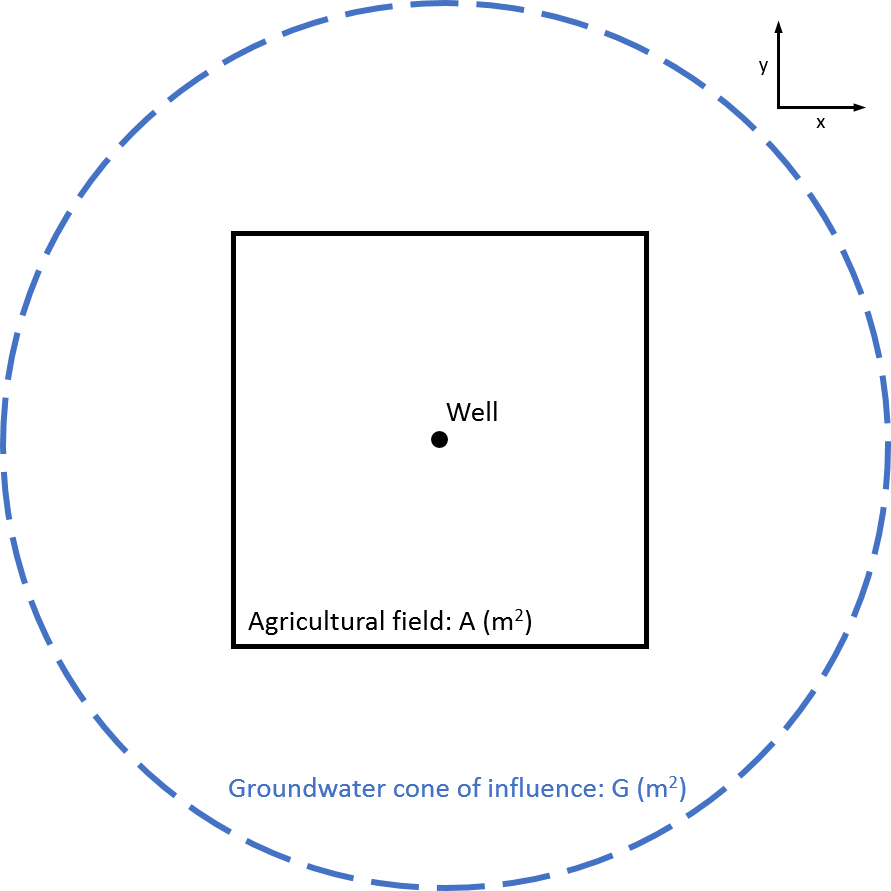
\includegraphics[width=0.4\linewidth]{Crop_cover}
% \captionsetup{justification=centering}
% \caption{Fictive schematic of crop cover area (C$_\%$)}
% \label{fig:Crop_cover}
%\end{figure}
%
%The A over G ratio ($C_{\%}$) shows top-view perspectives of spatially concatenated multiplication of agricultural fields, as visualized in Figure (\ref{fig:Crop_cover}). High $C_{\%}$ values (close to one) suggest the implementation of agricultural fields is possible at close mutual distance. \\
%
%\begin{equation}
% C_{\%} = \frac{A}{G}
%\label{eq:RR}
%\end{equation}
%
%Where  C$_{\%}$ is the crop cover ratio (-), $A$ (m$^2$) is the crop specific agricultural field size and $G$ (m$^2$) is the areal groundwater cone of influence. \\

\textbf{Financial yield} \\
Based on the described crop specification, the simulated water volumes withdrawn can be expressed in financial returns. The agricultural yield (kg/m$^3$) and the weighted crop prices (GHS/kg) are defined. From consistence considerations it is chosen to express the financial returns in US dollars. The July 7$th$ Bloomberg financial exchange rate is applied: 0.2081 USD/GHS \citep{Bloomberg2018}.

\subsection{Costs - water withdrawal}
The ASR system profits are accompanied by costs. For this research all Capital Expenditures(CAPEX) are unknown and ignored. The same applies for large parts of the Operating Expenses (OPEX), e.g. farmer wage and fertilizer costs. The only costs accounted in this research are the costs related to the energy (diesel) consumption due to pumping. Outcomes are purely focused on the feasibility of the daily system operation. An impression is generated, whether or not regular ASR-system operation on its own is profitable. \\

\begin{figure}[h!]
 \centering
 
\includegraphics[width=0.35\linewidth]{Schematic_pump_costs}
 \captionsetup{justification=centering} 
 \caption[Schematic of the ASR system operational pumping costs]{Schematic of the ASR system operational pumping costs \\ (visual support by Nociconist, Quan Do and Phonlaphat Throngsriphong from Noun Project - \url{https://thenounproject.com})}
 \label{fig:Schematic_pump_costs}
\end{figure}

\textbf{Synthetic pump application} \\
The Pedrollo 4" submergence pump is applied in fieldwork measurements. The same pump, i.e. its specifications, is used a standard in the subsequent parts of research. General specification can be found in Appendix \ref{chapter:Pedrollo_product_specs}. The results of the synthetic simulations contains time dependent (4 hours daily, 243 days) discharge rates. As soon as the maximum pumping capacity is exceeded (at any moment), it is assumed the specific dry season simulation is carried out by the implementation of (one or more) extra (same) pump(s). By a parallel pump configuration the same heads and efficiencies are ensured, while discharge capacities are multiplied \citep{VandeGiesen2013}. \\ 
%As soon as the maximum pumping capacity is exceeded by the obtained (simulated) discharge rates (results Chapter \ref{chapter:model_scenarios}),

\textbf{Energy Consumption} \\
The available groundwater has to be lifted to the surface. Depends on the obtained discharges, the lifting action requires a certain magnitude of power (Equation \ref{N_net}). For water displacement the difference between pump position and surface level (30m) is retained. An extra lift of 15 m is added to account for friction losses and the higher position (above surface) of the poly tank(s). A total head lift of 45 m is applied.

\begin{equation}
N_{net} =  g * Q * \Delta H
\label{N_net}
\end{equation}

Where $N_{net}$ (kW) is the net power required, g (m/s$^2$) is the gravitational acceleration (9.81 m/s$^2$), Q (m$^3$/s) is the dry season discharge (time dependent (and in seconds)) and $\Delta$H (m) is the net head (total lift) required. In this equation it is assumed the water has a density of 1000 kg/m$^3$. \\

In general, the use of power gets accompanied by losses (for example due to friction and turbulence). Ever single power-related equipment works at a certain level of efficiency. The power generator applied in fieldwork (Appendix \ref{chapter:fieldwork_set-up}) is used over years. Due to its datedness, a generator efficiency of 70\% is estimated. The efficiency of the Pedrollo pump(s) is dependent on the discharge rate during dry season operation. An overview of the efficiency curve is present in Appendix \ref{chapter:Pedrollo_product_specs}. In this study, the pump efficiencies are related to the time dependent discharges obtained in the synthetic model simulations. Besides equipment losses, energy get lost due to mutual transmission. An extra efficiency value of 90\% is accounted \citep{VandeGiesen2013}. Result is a variable ASR system efficiency that never exceeds 36.5 \% (based on the maximum pump efficiency of 58\%).

\begin{equation}
 \eta_{total} =   \eta_{generator} * \eta_{transmission} * \eta_{pump} \end{equation}

Where $\eta_{total}$ (-) is the overall power efficiency, $\eta_{generator}$ (-) is the generator power efficiency, $\eta_{transmission}$ (-) is the transmission power efficiency and $\eta_{pump}$ (-) is the pump power efficiency. \\

The combination of total ASR-system efficiency and net required power results in a gross power (Equation \ref{Eq:gross}). The gross power should be delivered by the generator to gain the desired volumes of water at the agricultural fields. Multiplying the gross power required by the total hours of pump operation returns the total energy consumed (kWh).

\begin{equation}
 N_{gross} =   \frac{N_{net}}{\eta_{total}}
\label{Eq:gross}
\end{equation}

Where $N_{gross}$ (kW) is the gross power required, $N_{net}$ (kW) is the net power required and $\eta_{total}$ (-) is the overall power efficiency. \\

\textbf{Energy costs} \\
The Kipor power generator (Appendix \ref{chapter:fieldwork_set-up}) contains a 15 liter diesel tank. On a fully filled tank the generator can operate for 6.5 hours. A fuel consumption of 2.31 l/h is taken into account. During operation the generator delivers a continuous power capacity of 4.5 kW \citep{TS242018}. The Ghana diesel price of 5.03 GHS/l (begin of July 2018) is adopted as normative \citep{GlobalPetrolPrices2018}. The Bloomberg financial exchange rate (0.2081 USD/GHS) is also applied on the fuel costs for proper financial comparison \citep{Bloomberg2018}.

\begin{equation}
 Cost_{fuel} =  \frac{consump_{gen} * price_{fuel} * rate_{exchange}}{power_{gen}}
\end{equation}

Where $Cost_{fuel}$ (USD/kWh) is the price of fuel,  $consump_{gen}$ (l/h) is the generator fuel consumption,  $price_{fuel}$ (GHS/l) is the fuel price in Ghana, $rate_{exchange}$ (USD/GHS) is the Bloomberg financial currency rate and $power_{gen}$ (kW) is the generator continuous power capacity. \\

\section{Financial yield}
\label{section:fin_yield}
The impact of the different ASR system improvements are (amongst others) expressed in terms of total volumes discharged (Section \ref{subsec:improvements}). These volumes are the summed-up results of eight months daily groundwater withdrawal, where discharge rates are limited due to the set bound in GWT drawdown (14 m). The time dependent discharge volumes of the first four months (120 days) are allocated for the production of tomatoes (one cropping season). The groundwater withdrawal of the subsequent 123 days of dry season is assigned to a single cycle of groundnut cultivation. The corresponding financial yields are acquired by subjecting the obtained water quantities to the volume-to-yield methods (described in Section \ref{subsec:Yield_crop}). The crop-specific financial results are for each soil scenario and for each type of ASR system improvement (multiple steps) presented in Figure \ref{fig:tom_yield} (Tomatoes) and Figure \ref{fig:gn_yield} (Groundnut). \\

The determination of the financial yield is based on highly simplistic methods. The obtained revenues are purely based on a crop-specific factorization of the derived discharge volumes. Therefore, the (improved) ASR system revenue (USD) patterns are in line with the prior presented total discharge volumes (m$^3$). The results show that higher (financial) yield can be expected by the implementation of the explored types of ASR system improvement. Exact revenues are dependent on the type and 'size' of improvement. The financial yield of the synthetic base model (values on the Figures absolute left-side) is utmost somewhat more than doubled by the explored research scope of system improvements. \\

%* The obtained results are all based on volume-to-yield transformations described in Section \ref{section:Theory_yields}. \\
%%\subsection{Financial yield}

 \begin{figure}[h!]
 \centering
 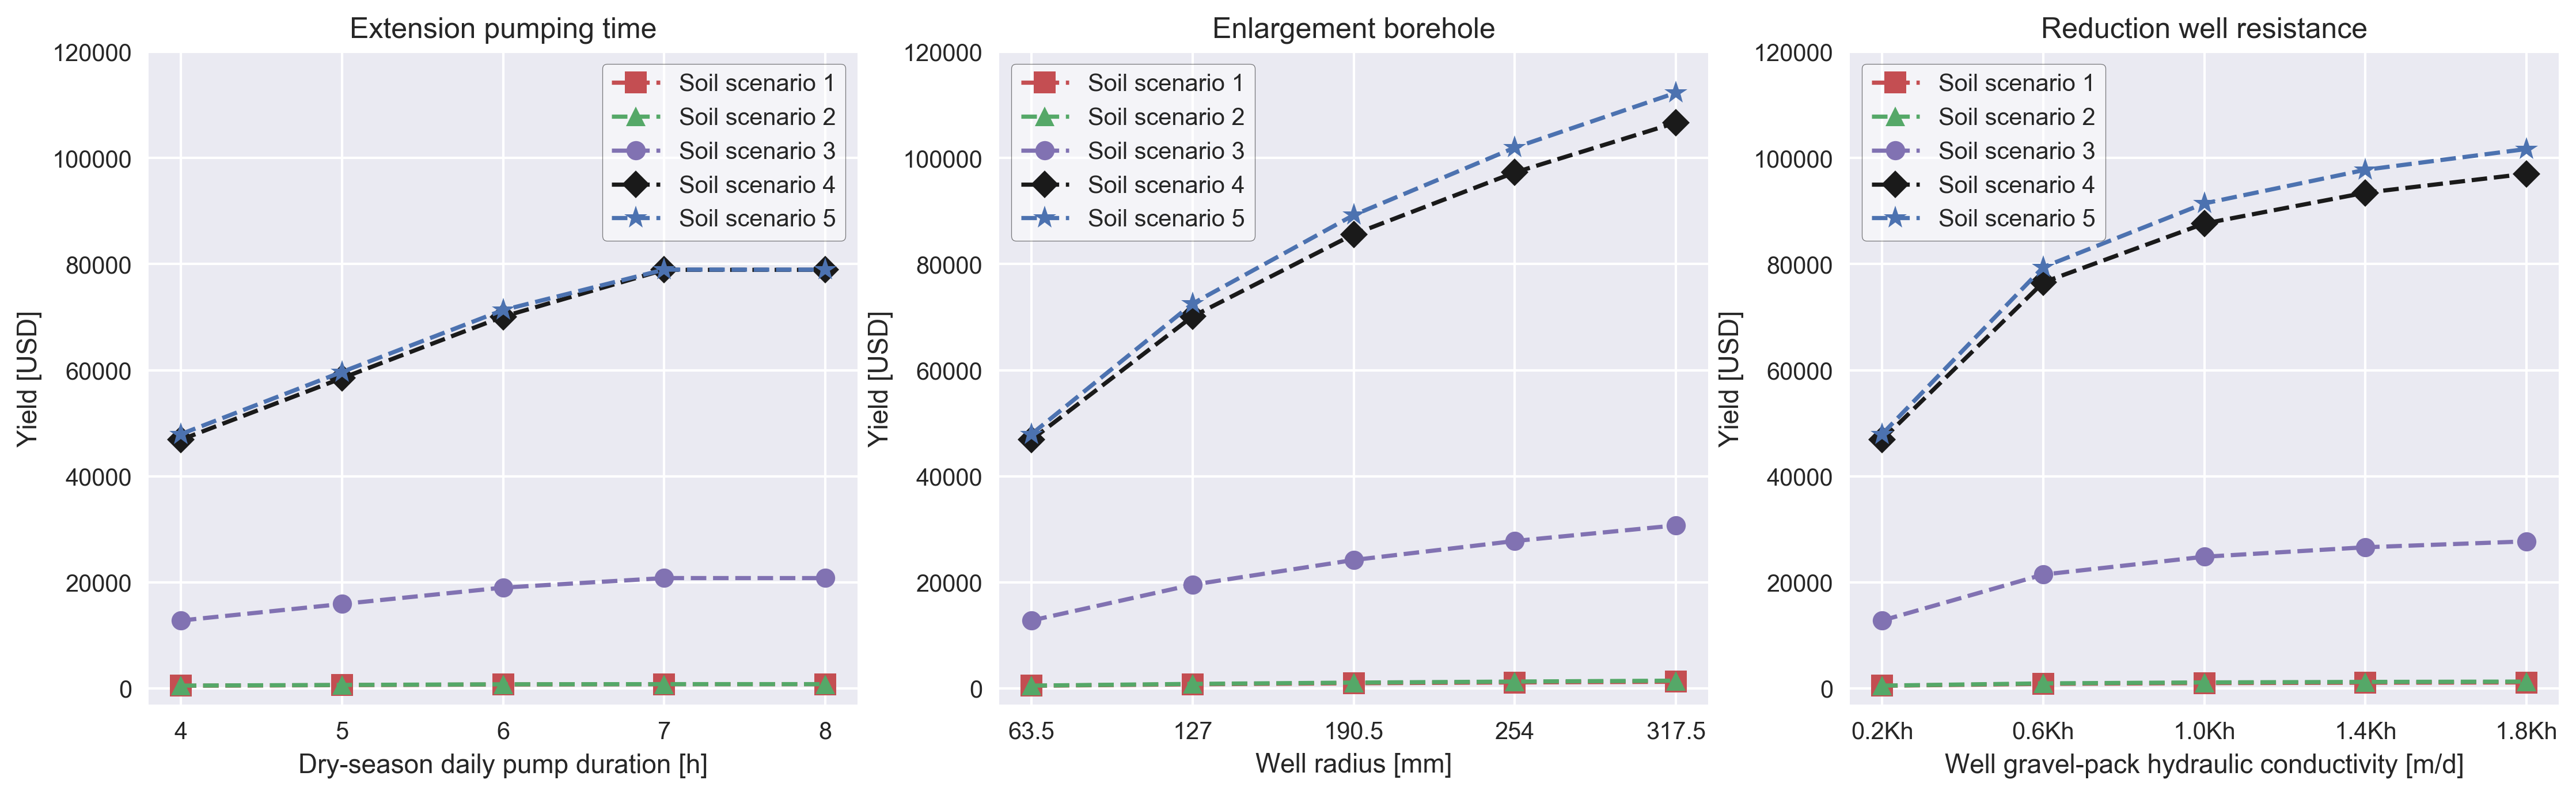
\includegraphics[width=1.0\linewidth]{tom_yield}
 \captionsetup{justification=centering} 
 \caption{Financial yield - Tomatoes (4 months) - three types of ASR system improvement}
 \label{fig:tom_yield}
\end{figure}

\begin{figure}[H]
 \centering
 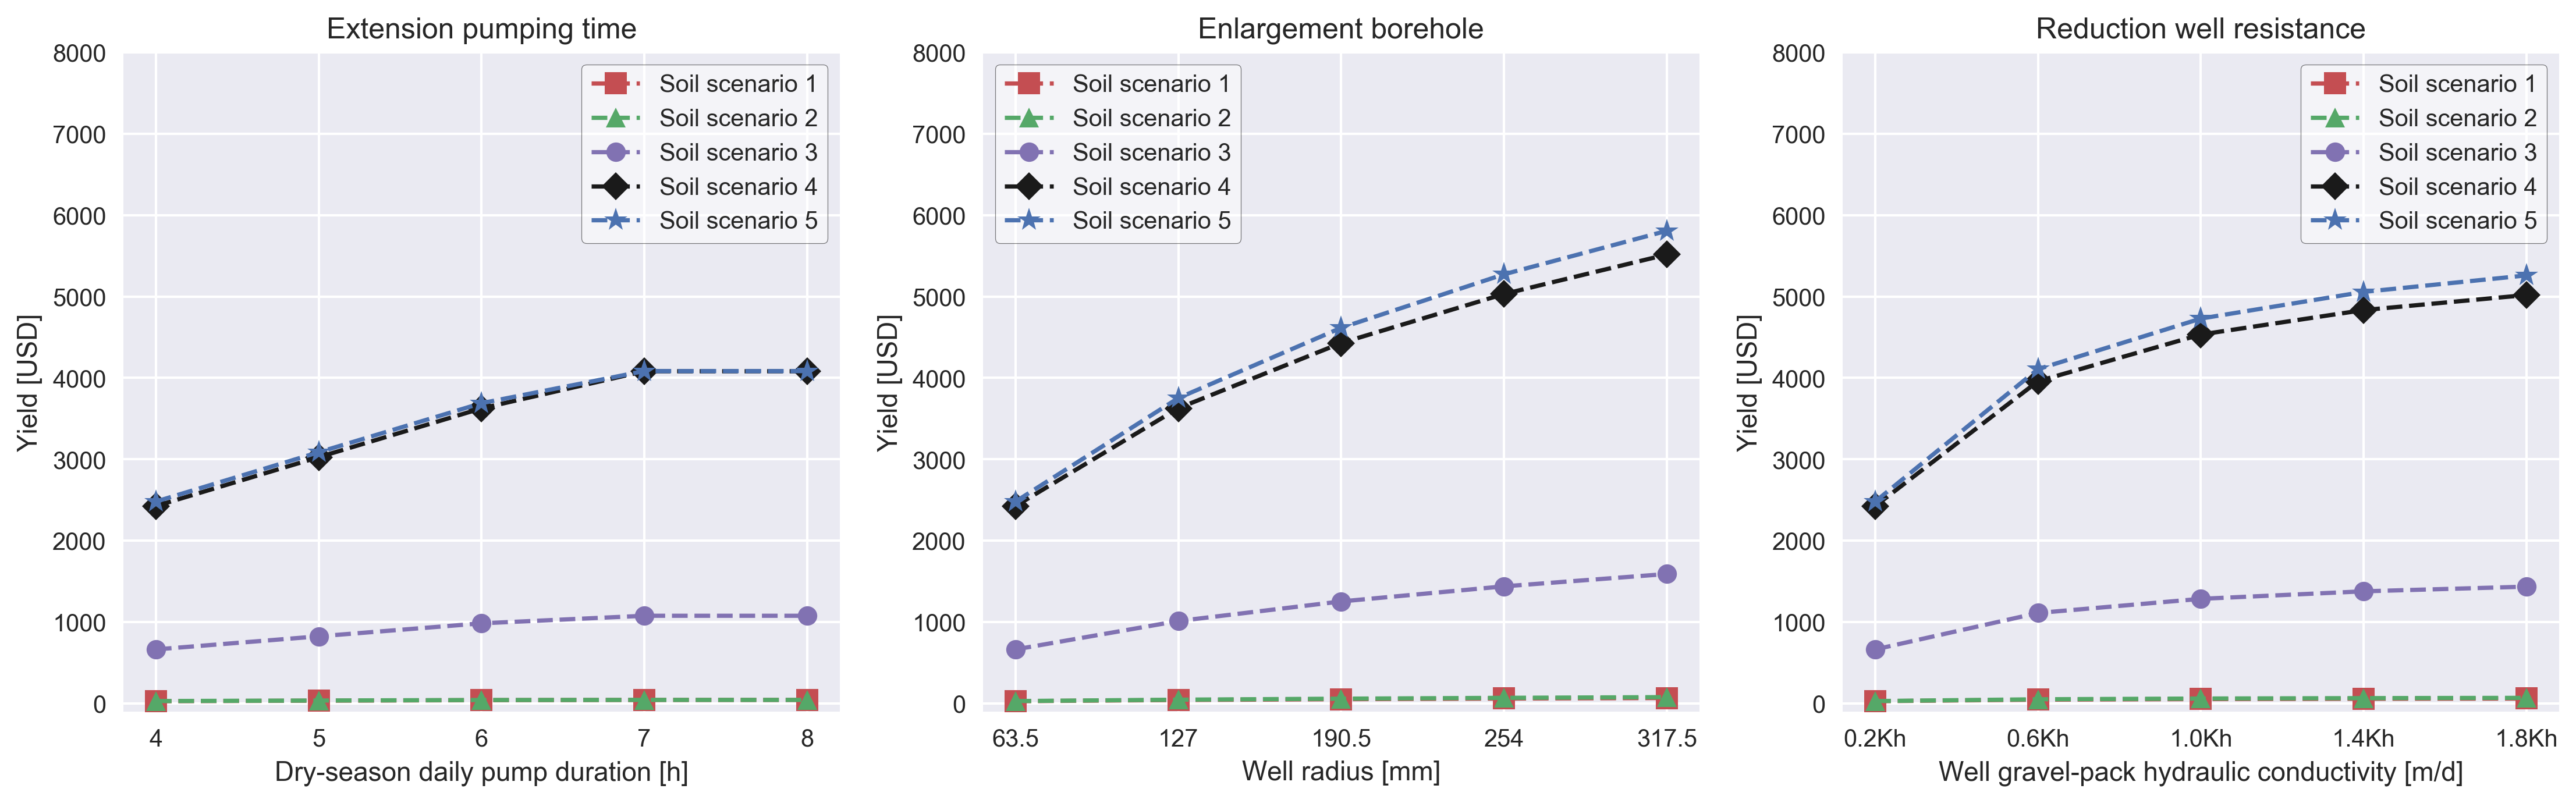
\includegraphics[width=1.0\linewidth]{gn_yield}
 \captionsetup{justification=centering} 
 \caption{Financial yield - Groundnut (4 months) - three types of ASR system improvement}
 \label{fig:gn_yield}
\end{figure}

The dry season use of an ASR system is simulated by temporal but daily pump operation. The discharge performances are more or less daily repetitive (Figure \ref{fig:Example_Sc3_base_discharge}). Significant differences in the total volumes of water withdrawn are absent between days. The water allocation for the cultivation of tomatoes versus groundnut is quantitatively comparable. Nonetheless, a comparison between the Figures \ref{fig:tom_yield} and \ref{fig:gn_yield} reveals that the crop-specific revenues substantially differ. A glimpse at the figures Y-axes (different yield values) gives clarity. Independently of the type of system improvement, the tomato revenues considerably exceed the groundnut revenues (about 15 - 20 times higher). The results show, it can pay-off to pick the ‘right’ crop. The determination of the cultivated crop type potentially affects the ASR system financial profits more dominantly, than the implementation of one of the system improvements explored in the scope of this research. \\

%The available water volumes are approximately the same for the first four months (tomatoes) and the subsequent four months (groundnut) of dry season. Nonetheless, the obtained yield differ strongly. Note, the y-axis of Figure \ref{fig:tom_yield} and Figure \ref{fig:gn_yield} are not the same. The obtained financial yield is highly dependent on the crop of interest and its transfer assumptions. \\

%The tomato crop can be labelled as a potential high-profitable crop. 
%The obtained (time dependent) discharge volumes of the different types of ASR system improvements are subjected to the methodologies on financial yield.

It is worth-mentioning that the derivation method of the financial yield is not only simplistic, but also highly uncertain. The obtained financial results should only be interpreted as indicative. As mentioned in the crop specification (Section \ref{subsec:Yield_crop}), yields can differ both in terms of agriculture (tons per hectare) and financially (GHS per kilogram). The revenues are strongly dependent on aspects as crop quality, shelf life and seasonal crop availability. The market (fluctuation) is decisive in the crop-specific (wholesale)price. Therefore, it remains to a certain extent questionable which crop type is 'right'. If more detailed information on the combination of crop revenues and ASR system implementation is desired, additional research is advisable. \\

%\begin{figure}[h!]
% \centering
% 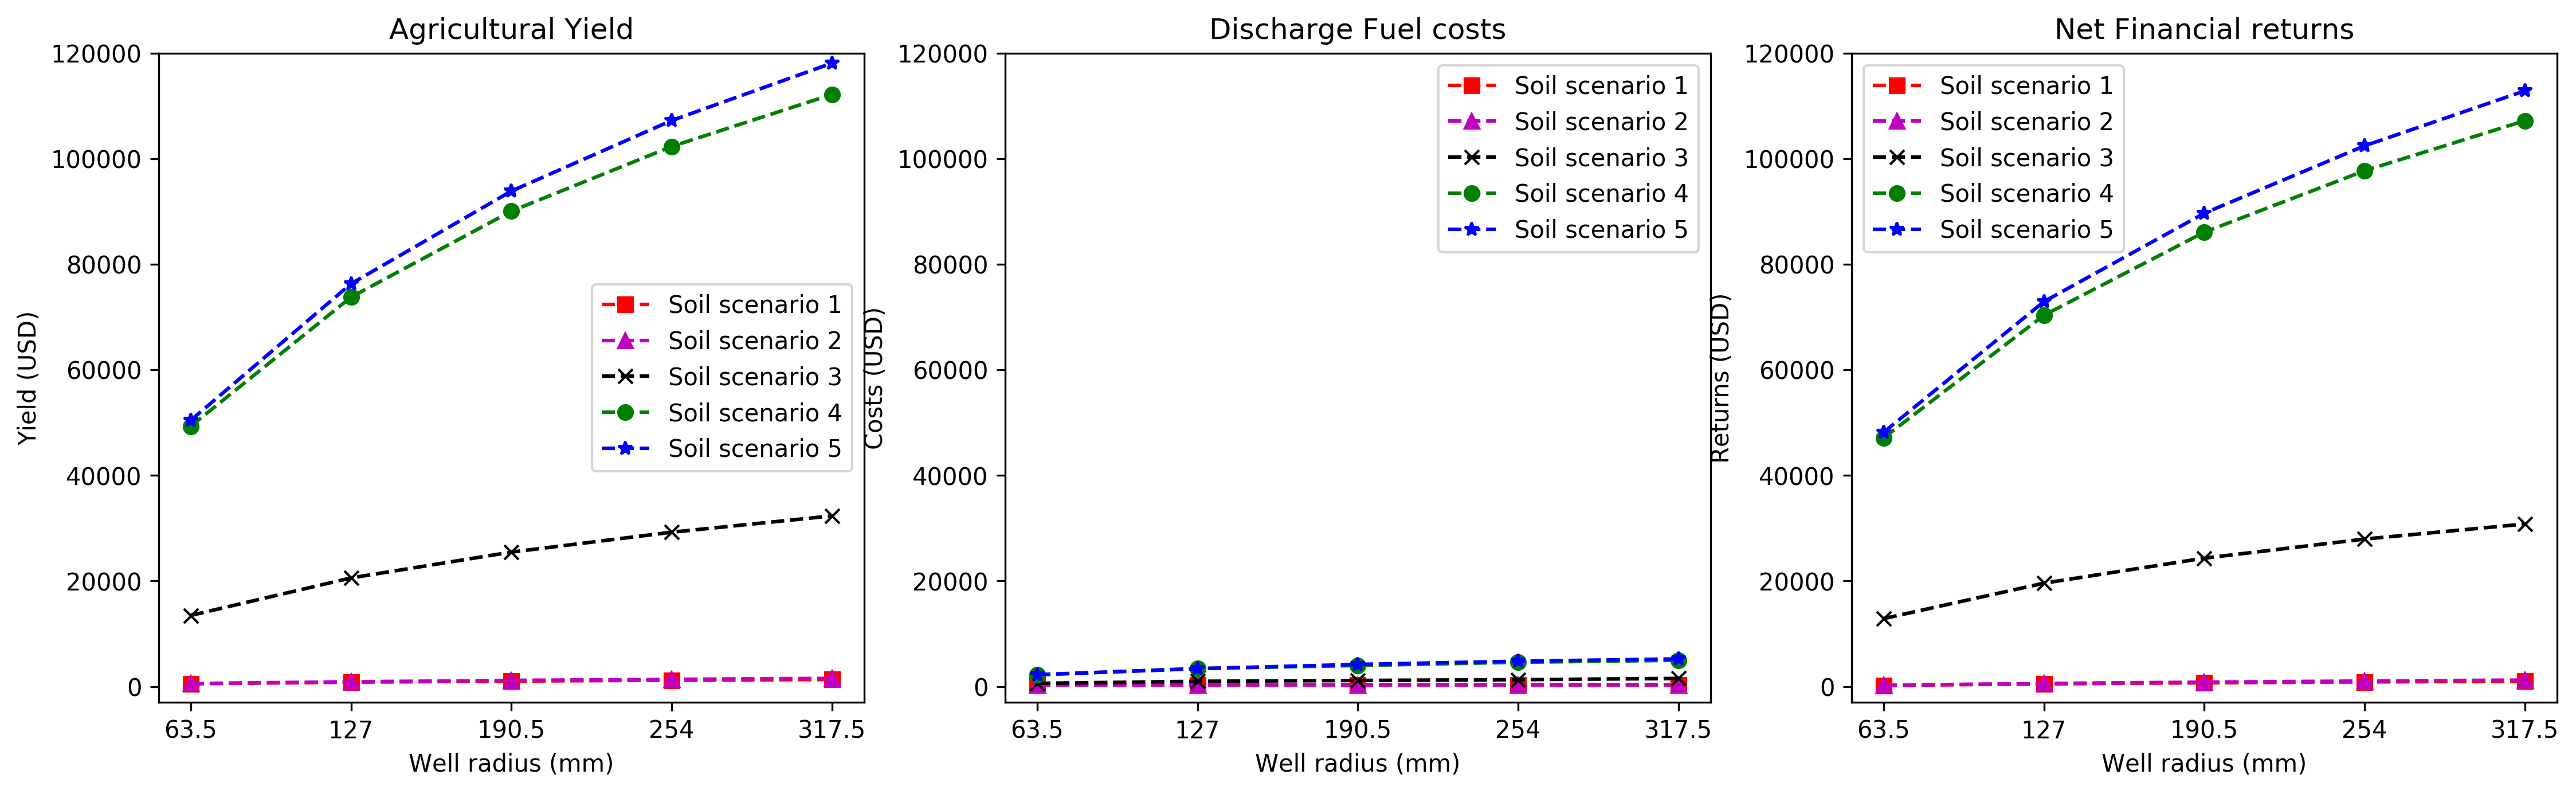
\includegraphics[width=1.0\linewidth]{Results_financial_up_diam}
% \captionsetup{justification=centering} 
% \caption{Well diameter upscaling dependent results on net agricultural yield, costs and net returns}
% \label{fig:Results_financial_up_diam}
%\end{figure}
%
%\begin{figure}[h!]
% \centering
% 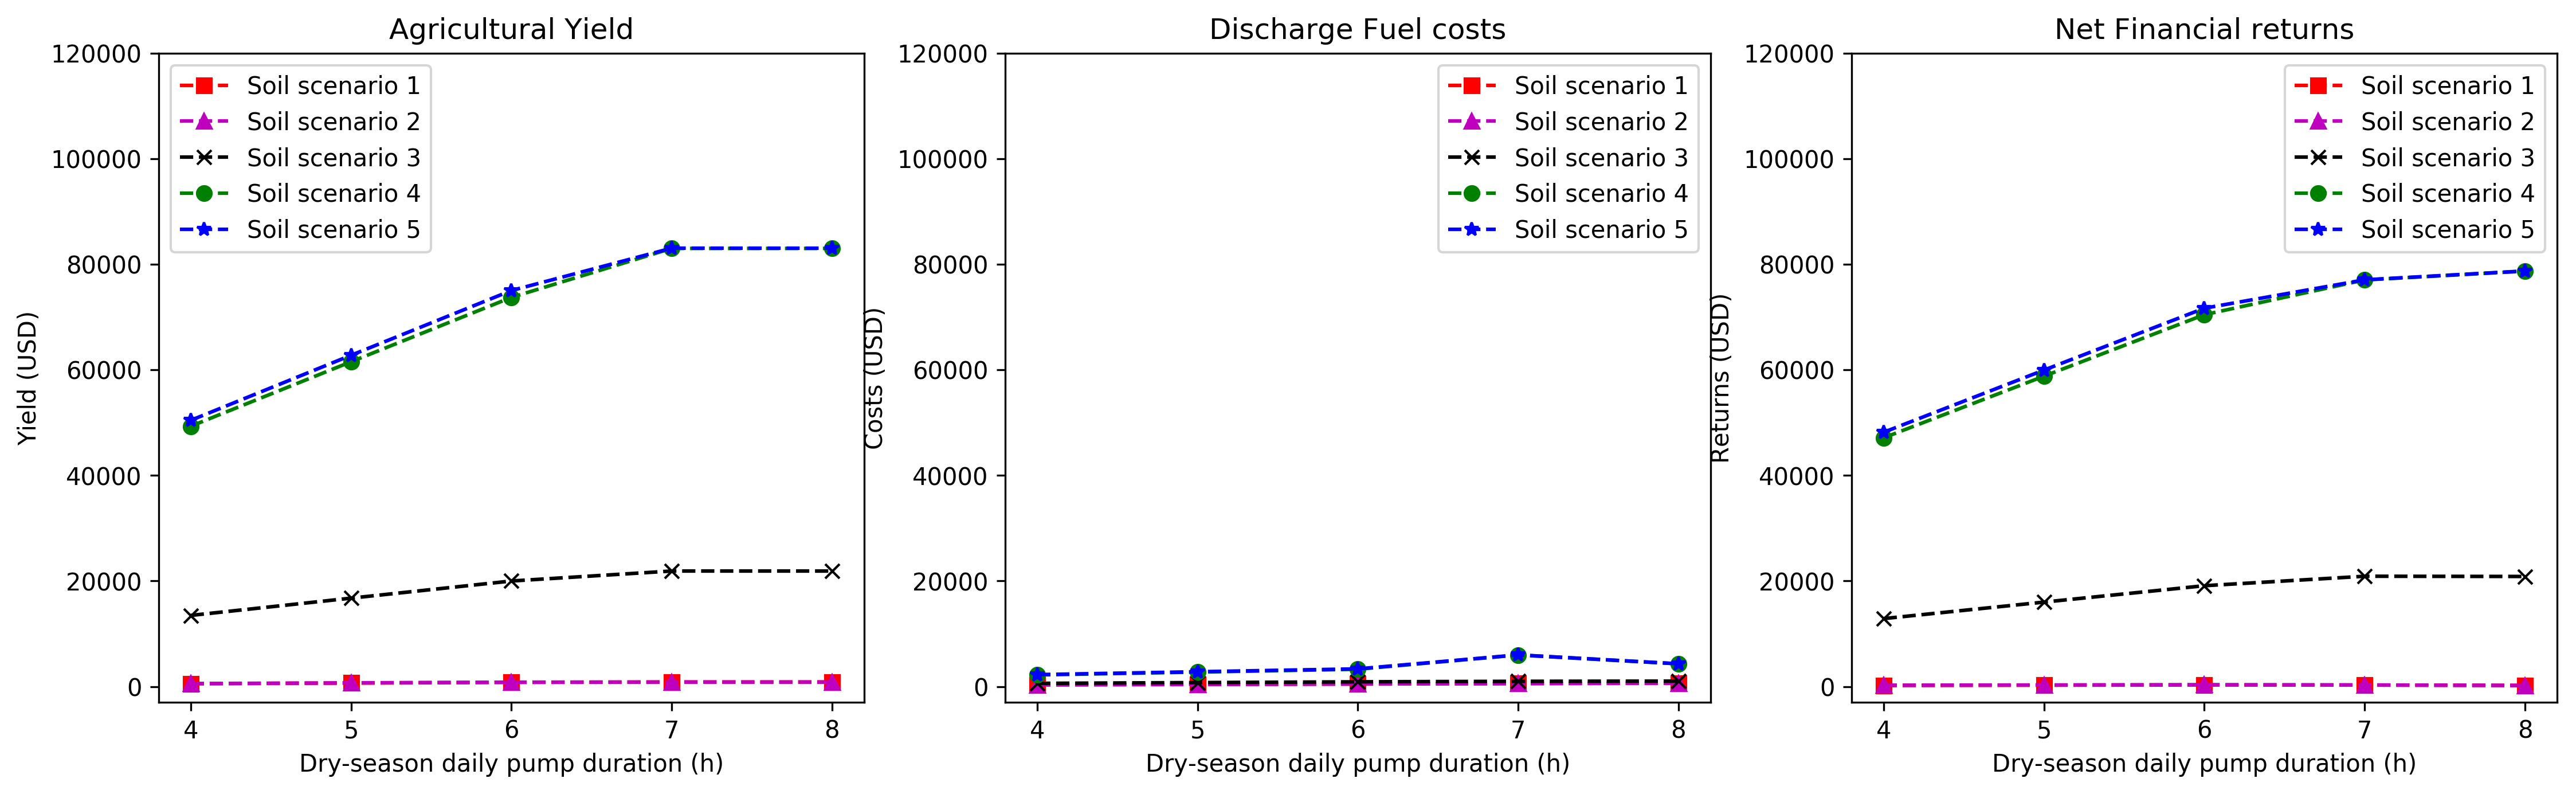
\includegraphics[width=1.0\linewidth]{Results_financial_up_time}
% \captionsetup{justification=centering} 
% \caption{time enlarged results on net agricultural yield, costs and net returns}
% \label{fig:Results_financial_up_time}
%\end{figure}
%
%\begin{figure}[h!]
% \centering
% 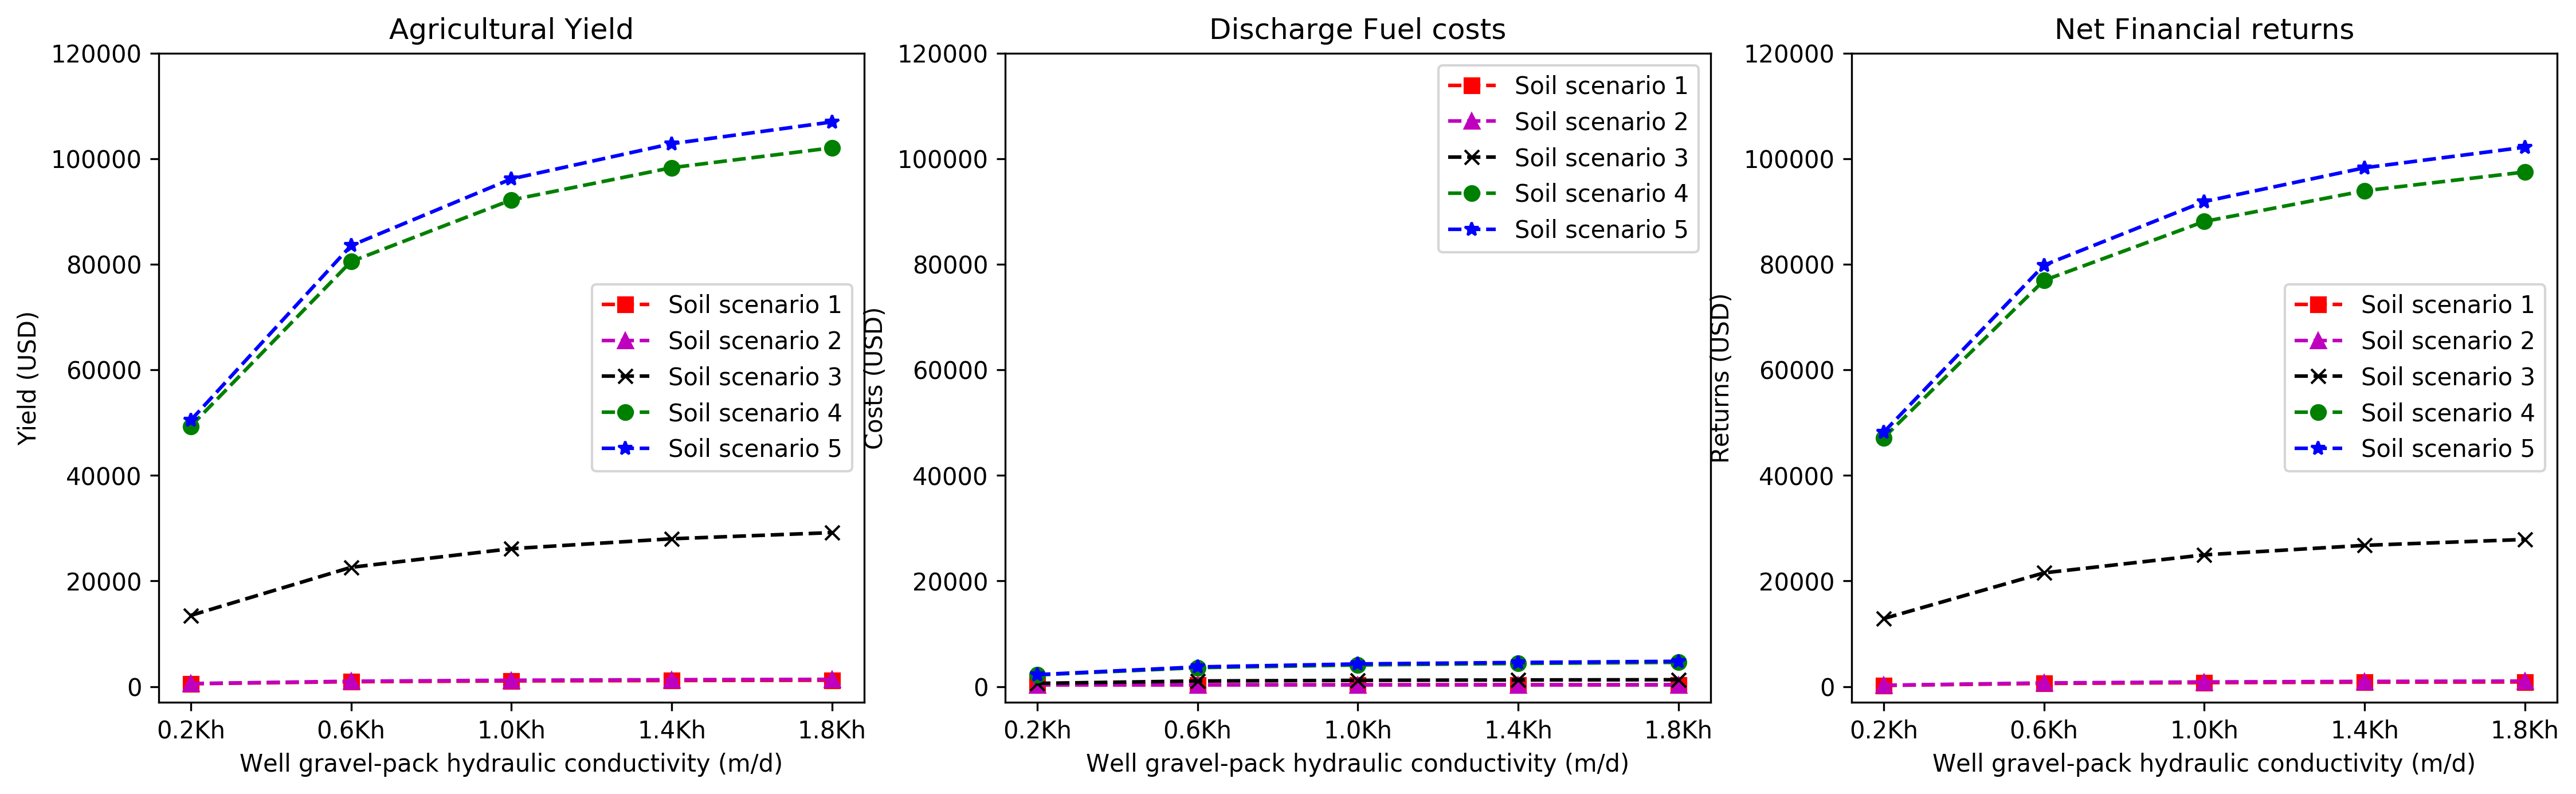
\includegraphics[width=1.0\linewidth]{Results_financial_up_screen}
% \captionsetup{justification=centering} 
% \caption{screen improved results on net agricultural yield, costs and net returns}
% \label{fig:Results_financial_up_screen}
%\end{figure}

\section{Pumping costs}
\label{section:pump_costs}
By the introduction of this section, the acquired ASR system revenues are accompanied by system operational costs. The costs included, are the expenses incurred by the generator diesel fuel consumption (daily pump operation). The remainder of CAPEX (e.g. system installation and pump purchase) and OPEX (e.g. farmer loans and fertilizer costs) is ignored. In northern Ghana practical ASR system implementation it is not unthinkable that elements (e.g. pump and borehole installation) and costs are optimally covered by funds. Nevertheless, the pumping costs are predominantly included to give solely an impression of the (improved) operational feasibility of an ASR system in northern Ghana. \\

The costs for the withdrawal of groundwater (total volumes presented in Section \ref{subsec:improvements}) are for each soil scenario and for each type of ASR system improvement (multiple steps) presented in Figure \ref{fig:tom_gn_yield}. For the simulation of eight months of daily discharge, the operational costs may reach from hundreds upto thousands of dollars (dependent on the volumes and conditions). Herewith, the operational expenses (eight months) are minor relative to the obtained tomato yields, but quantitatively comparable with the revenues of a single groundnut cropping season. 

\begin{figure}[h!]
 \centering
 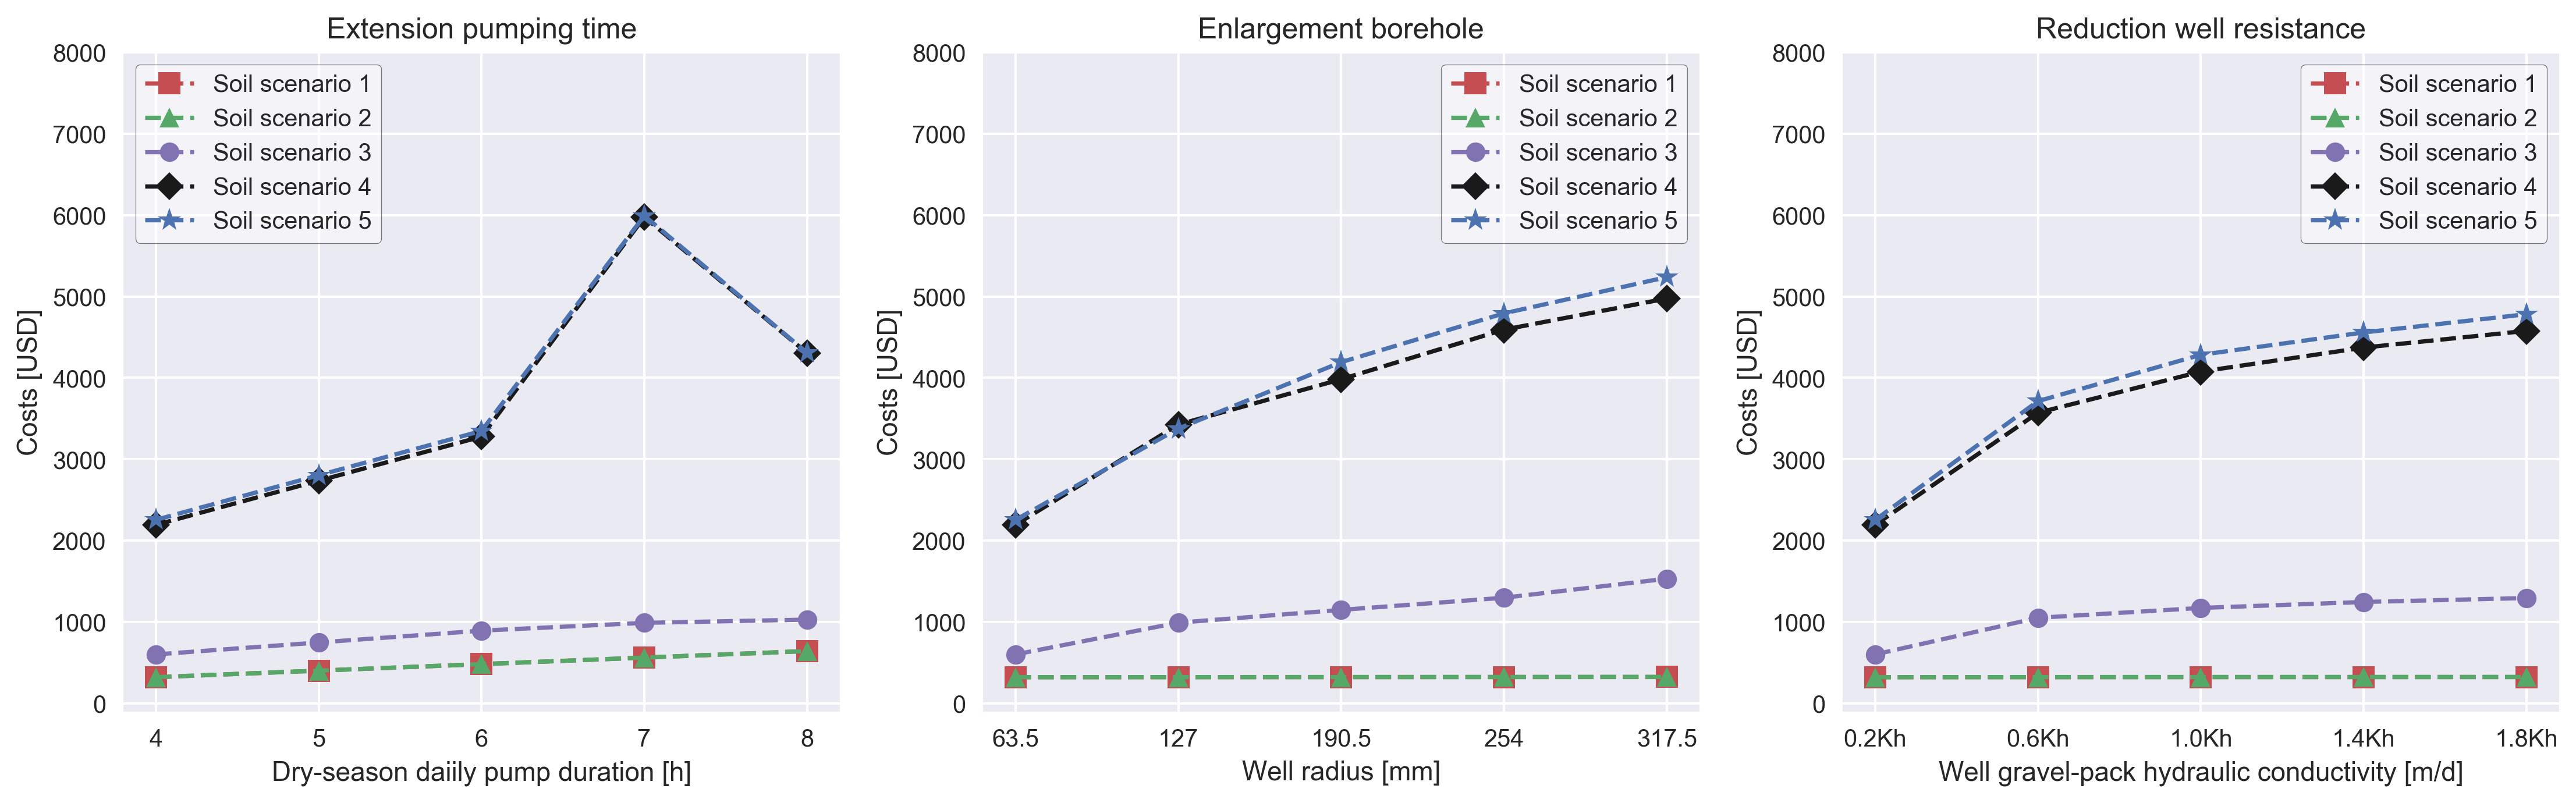
\includegraphics[width=1.0\linewidth]{tom_gn_costs}
 \captionsetup{justification=centering} 
 \caption{Pumping costs - dry season (8 months) - three types of ASR system improvement}
 \label{fig:tom_gn_yield}
\end{figure}

In the comparison of the soil scenario 1 and 2 versus soil scenario 3 substantial deviations are present in the simulated total volumes discharged (Section \ref{subsec:improvements}). As visible in Figure \ref{fig:tom_gn_yield}, these deviations are less dominantly present in the pumping costs. This is most clearly visible for the base model simulations (absolute left-side of Figures) and the simulations with an ('improved') extension of the daily pumping time. The reduced deviation in costs can be attributed to the applied pump efficiencies. The pumping curve of the Pedrollo 4" submersible pump is defined as normative (Appendix \ref{chapter:Pedrollo_product_specs}). The discharge rates obtained in the simulations of soil scenarios 1 and 2 do not ideally match the specification of this pump. As a result, low(er) pumping efficiencies are implemented and high(er) discharge costs are sorted. \\

%The obtained (model) discharges for the soil scenarios 1 and 2 are extremely low. As a consequence, pumping efficiencies (Pedrollo 4" submergence pumping curve) are stated to be almost zero. A situation highly unlikely. In practise, a specific pump type will be applied that suits the circumstances. As a consequence, unrealistic judgements and comparisons are applied.

Besides, the Pedrollo 4" submersible pump has, like every pump, its own specific discharge limits. The obtained discharge rates for the soil scenario 4 and 5 simulations (base model and improved system) are out of pumping range. An inconvenience, worked around by the (simulated) installation of one or more additional pumps. By this approach the specified discharge rates are (theoretically) met. As an adverse affect, moderate pumping efficiencies can occur when the number of pumps is stepped up. Herewith, the outliers (peak) in operational cost for the soil scenario 4 and 5 ('improved') seven hour daily pumping operation (Figure \ref{fig:tom_gn_yield}) can be justified. \\  

%Note, the outlier in the soil scenarios 4 and 5 for the situation of 7 hours pumping operation can be justified by the application of an unfortunate number of pumps. Efficiencies are in this particular case relatively low (as low as 35\%). \\

The installation of a too powerful pump and the use of abundant number of pumps (in parallel) are both situations that are practically unlikely and undesired (low efficiencies and high purchase costs). Figure \ref{fig:tom_gn_yield_maxeff} presents the ASR system operational costs for each soil scenario and for each type of improvement (multiple steps), when maximum pumping efficiencies are taken into account. Based on the specifications of the Pedrollo 4" submersible pump a maximum pumping efficiency of 58\% is implemented (Appendix \ref{chapter:Pedrollo_product_specs}). A comparison of the Figures \ref{fig:tom_gn_yield} and \ref{fig:tom_gn_yield_maxeff} learns, optimal pumping efficiencies can (sometimes) significantly lower the systems operational costs. For a high efficient use of the ASR system, one should tune the applied pump (pumping curve) to the local circumstances. 

%Substantial deviations in the total groundwater withdrawn volumes (Section \ref{subsec:improvements}) are (amongst others) present between the soil scenario 1, 2 and soil scenario 3.

%Two developments present in the results of Figure \ref{fig:tom_gn_yield} require a specification. Despite the substantial deviation in total volumes withdrawn (Section \ref{subsec:improvements}), the base model operational costs (absolute left-side in Figures) for the soil scenarios 1 and 2 do not deviate much from the costs to obtain the water volumes in soil scenario 3.

%However, the increase in pump numbers is not reflected in this research costs. As a consequence, unrealistic judgements and comparisons are applied. \\

%can be attributed to an inconvenient change in the number of pumps required to deliver the specified discharge rates. 

\begin{figure}[h!]
 \centering
 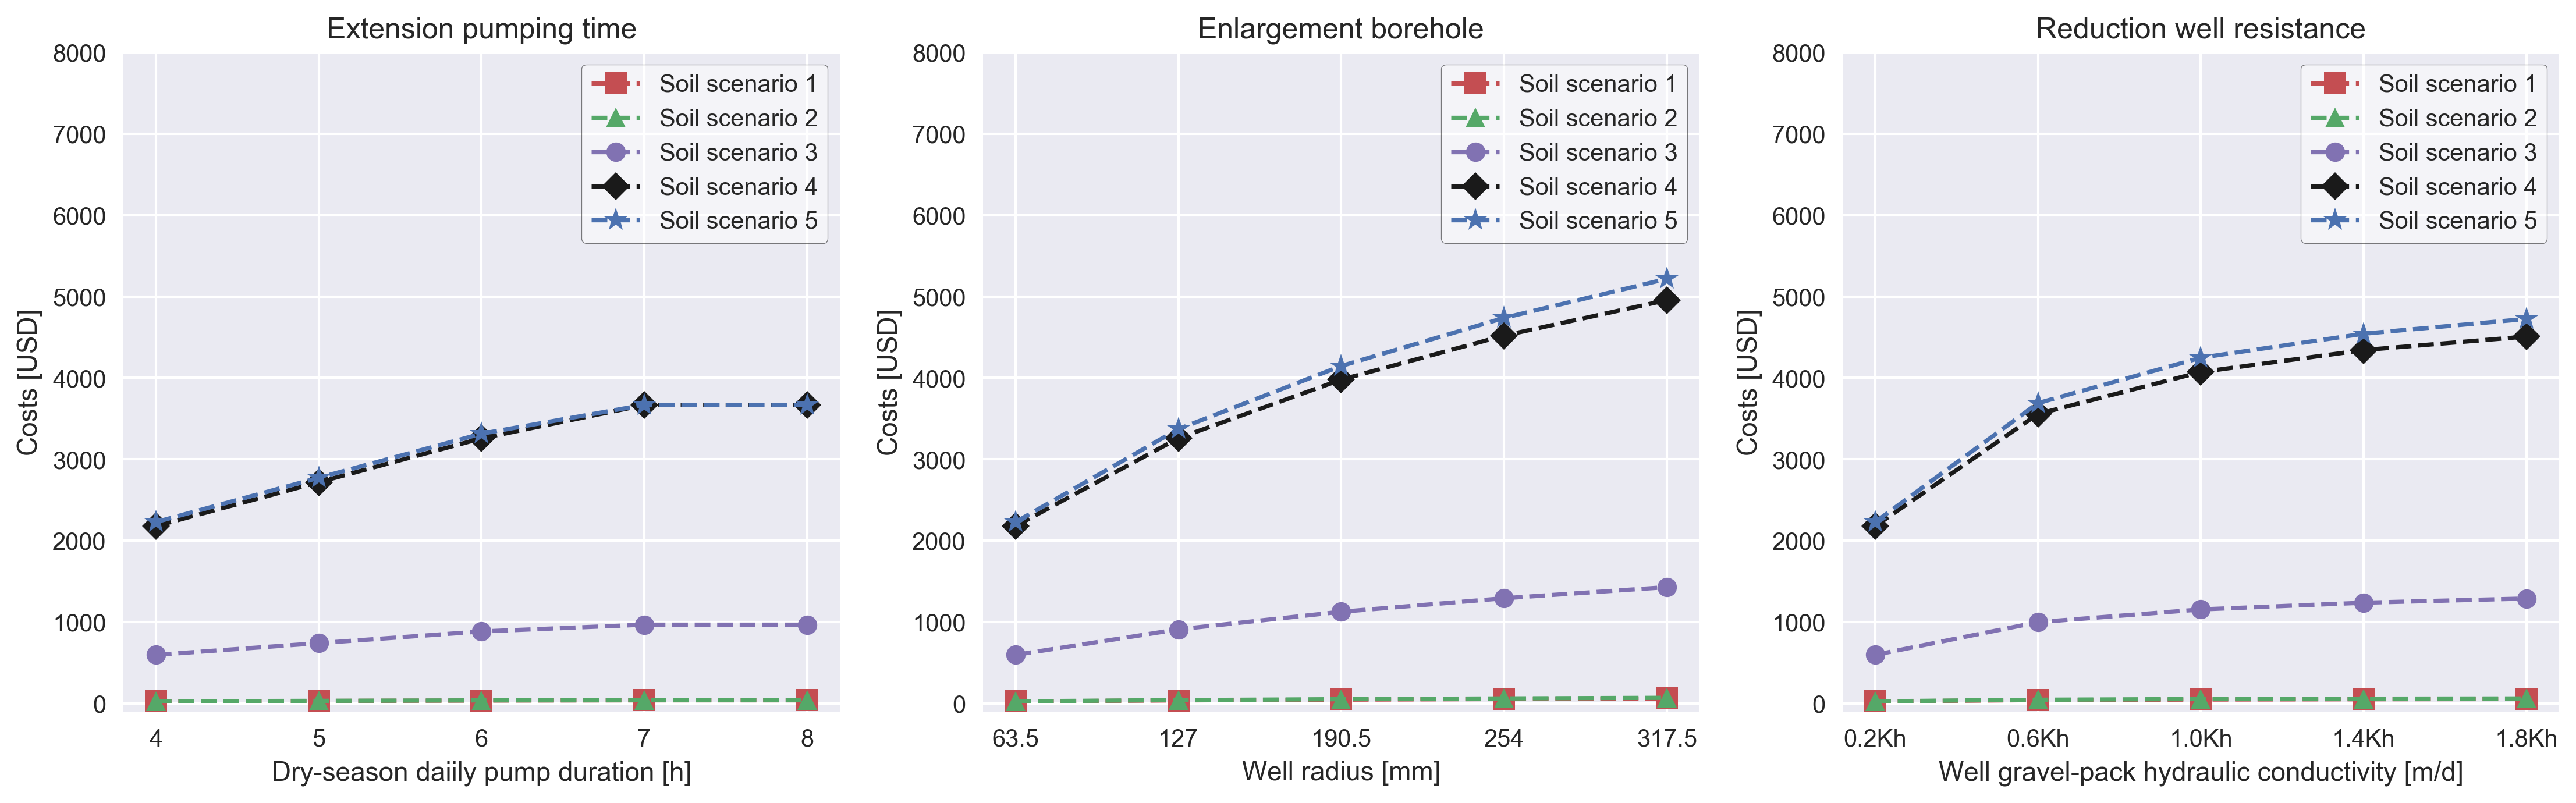
\includegraphics[width=1.0\linewidth]{tom_gn_costs_maxeff}
 \captionsetup{justification=centering} 
 \caption{Pumping costs - maximum pumping efficiency - dry season (8 months) - three types of ASR system improvement}
 \label{fig:tom_gn_yield_maxeff}
\end{figure}

An overview of the business case financial returns is presented in Appendix \ref{section:bus_case}. The ASR system financial returns for both, the 'actual' and the optimal pumping efficiency costs are included. \\ 

%
%note, the remainder of OPEX and CAPEX is undetermined. deze kosten kunnen echter deels opgevangen worden door europese fondsen (niet ondenkbaar). Daardoor wordt de  costs are undetermined. 
%
% Therefore, the business case is not quite representative for the actual het zegt alleen solely mogelijk iets over het (beter kunnen) gebruik van het ASR system in northern Ghana. 
% 
%door de afwezigheid van dan en dat niet bepaald een business case. maar tegelijkertijd toch ook weer wel. sommige items kunnen mogelijk vergoeding krijgen vanuit (europese) fondsen. Waardoor de financial balance al weer iets representatiever geinterpreteerd kan worden. 
%
% due solely the withdrawal of water,
% gekozen voor een zeer onrealistische financiele situatie, omdat informatie gewoon afwezig is. capex (denk aan pomp costen zelf. plaatsing van de well, land, irigatie systeem, polytanks) opex (denk aan famers loans, fertilizers) Bovendien kunnen onderdelen vanuit (europese) fondsen in aanmerking komen voor een fianciele compensatie. waardoor het financiele kostenplaatje al weer iets minder onrealistisch is. nonetheless, business case blijft hoogst onzeker. verder onderzoek dan ook zeker wenselijk. 

\section{Results \& conclusions}
\label{section:Yields_conclusions}
This section contains the conclusions that can be drawn from the ASR system business case. Key options concerning the agricultural yield and pumping costs are stated, to guarantee efficient (financial) system handling. \\

%and potentially improve the system's financial feasibility. \\

\begin{itemize}
\item{Yield increase} \\
By the implementation of the explored ASR system improvements, increased discharge volumes are acquired and higher financial (and agricultural) yield can be expected. A crop-specific yield comparison (Tomato versus Groundnut) reveals, the financial yield is potentially more dominantly affected by crop cultivation choice rather than the implementation of one of the investigated system improvements. Nonetheless, the crop-specific market price remains decisive in the ASR system financial feasibility.  

%met de juiste keuze in crop type kunnen de operational costs worden omgezet in profits. de system improvement kan hier een moderate role bij spelen, maar die invloed kan mogelijk wel net het verschil maken. (dit misschien in de discussie. hou het hier clinisch met kosten en opbrengsten). 

%Under the defined research conditions, it definitely pays-off to pick the ‘right’ crop. In terms of financial profit, the magnitude is more dominantly affected by crop choice, rather than ASR system improvements.

\item{Operational cost reduction} \\
The ASR system operational costs are influenced by the withdrawal efficiencies. For an efficient use of the ASR system, the applied pump (pumping curve) should be specifically tuned to the local possibilities in groundwater discharge rates. The natural geohydrological conditions and the system composition play a role in this process. The selection of the 'right' pump can make the difference in the financial feasibility of an ASR system. 

%Efficiencies are influenced by the achievable discharge rates (based on ASR system and soil conditions). Potential ASR system modifications and natural conditions play a role in this process. \\

\item{Additional research} \\
The business case contains strong simplifications, uncertainties and is far from complete. Multiple additional components in CAPEX and OPEX can be added. It is unknown to what extent ASR system components are eligible for funds. For a more detailed financial feasibility of an ASR system implemented in northern Ghana, future financial research is advisable. \\ 
\end{itemize}

%gekozen voor een zeer onrealistische financiele situatie, omdat informatie gewoon afwezig is. capex (denk aan pomp costen zelf. plaatsing van de well, land, irigatie systeem, polytanks) opex (denk aan famers loans, fertilizers) Bovendien kunnen onderdelen vanuit (europese) fondsen in aanmerking komen voor een fianciele compensatie. waardoor het financiele kostenplaatje al weer iets minder onrealistisch is. nonetheless, business case blijft hoogst onzeker. verder onderzoek dan ook zeker wenselijk. 

